	%%  A simple AAU report template.

%  2014-09-13 v. 1.1.0
%  Copyright 2010-2014 by Jesper Kjær Nielsen <jkn@es.aau.dk>
%
%  This is free software: you can redistribute it and/or modify
%  it under the terms of the GNU General Public License as published by
	%  the Free Software Foundation, either version 3 of the License, or
%  (at your option) any later version.
%
%  This is distributed in the hope that it will be useful,
%  but WITHOUT ANY WARRANTY; without even the implied warranty of
%  MERCHANTABILITY or FITNESS FOR A PARTICULAR PURPOSE.  See the
%  GNU General Public License for more details.
%
%  You can find the GNU General Public License at <http://www.gnu.org/licenses/>.
%
\input{setup/preamble.tex}% Package inclusion and set up of the document

\input{setup/hyphenations.tex}% Hypenation setup

\input{setup/macros.tex}% Macros

\begin{document}

\selectlanguage{english}

\pagestyle{empty}



%frontmatter
% Indholdsfortegnelse over kommentarer.
% HUSK AT SLETTE INDEN AFLEVERING! -->
%\pagenumbering{alph}
%\pdfbookmark[0]{Todoliste}{label:todos}
\listoftodos
\cleardoublepage
% <-- HUSK AT SLETTE INDEN AFLEVERING!

 %disable headers and footers
\pagenumbering{roman} %use roman page numbering in the frontmatter

%\pdfbookmark[0]{Forside}{label:forside}%
%\includepdf[fitpaper]{chapters/frontpage.pdf}
\input{chapters/frontpage}
\thispagestyle{empty}
{\small
\strut\vfill % push the content to the bottom of the page
\noindent Copyright \copyright{} \projectGroup{}, \projectFaculty{} \projectSemester{}, \AAU{} \the\year\par
\vspace{0.2cm}
\noindent This report is compiled in \LaTeX. Additionally is Mathworks MATLAB, Adobe Illustrator, Lucidcharts.com, Inkscape, and Autodesk Eagle used to draw figures, schematics, and charts.
}
\clearpage

\input{chapters/titlepages}

\cleardoublepage
\pagestyle{fancy} % Enable headers and footers again
\iflanguage{english}{
\chapter*{Preface\markboth{Preface}{Preface}}\label{ch:preface}%
\addcontentsline{toc}{chapter}{Preface}%
}{%
\chapter*{Forord\markboth{Forord}{Forord}}\label{ch:forord}%
\addcontentsline{toc}{chapter}{Forord}%
}
% Write here

\vspace{\baselineskip}\hfill \AAU, \today
\vfill\noindent
\begin{center}
\begin{minipage}[b]{0.45\textwidth}
 \centering
  \textit{John Doe}\\
  {\footnotesize <jodoe00@student.aau.dk>}
\end{minipage}

\end{center}


%\input{chapters/laesevejledning/_laesevejledning}


\begingroup % Let ToC start on even page.
  \let\cleardoublepage\clearevenpage
	\cleardoublepage
	\iflanguage{english}{\pdfbookmark[0]{Contents}{label:contents}}{\pdfbookmark[0]{Indhold}{label:indhold}}
 \tableofcontents
\endgroup

\cleardoublepage

\printnoidxglossaries

% Mainmatter
\pagenumbering{arabic} % Use arabic page numbering in the mainmatter

 % Include chapters
\chapter{Introduction}
The focus of this mini project is to implement and optimise a piece of Python code. 
In this case the code snippet consists of two functions used in process of image processing of images of the iris. The functions are a noise remover function and a histogram equalisation function. In the following sections the functionalities of the functions are elaborated and the setup and approach for the optimisation is outlined. 

\section{The Functions}
\label{sec:The_Functions}
The images which are processed by the two functions are normalised images of the iris as can be seen in \autoref{fig:SimPolar}. First the image is handled by the noise remover function and then the output is handled by the Equalise histogram function. The following sections describe the functionalities of the functions. 
\begin{figure}[h]
\centering
\includegraphics[width=\textwidth]{figures/002polar.jpg}
\caption{The normalised image of the iris before applying functions.}
\label{fig:SimPolar}
\end{figure}


\subsection{Noise Remover}
The purpose of the noise remover function is to remove noise occurring in the form of eyelashes covering parts of the iris. Usually the pixels showing the lashes will be among the darkest pixels. Since every image of the iris is different and how dark the iris is also varies, a threshold has to be identified adaptively. After the threshold has been found it is applied to all pixels in the image. If the pixels are lower than the threshold the pixels have to be eliminated and reconstructed from neighbouring pixels.
  
\subsection{Equalise Histogram}
This function has to identify the span of the "main" pixel values in the histogram. Once the "main" part of the  histogram has been identified this is stretched to cover the whole span of the range of the pixel values. This is done in order to increase the contrast in the image.  


\chapter{Research}
\label{cha:Research}

\section{Iris Recognition}
Modern iris recognition started in with an article by \cite{Daugman1993} discussing the security of using iris for recognition. An outline of how to do recognition was also laid out with the introduction of using  2D Gabor Waveletts to extract features of the complex pattern that can be found in an iris. This methodology has since been the basis for most iris recognition. It was also the foundation for IrisCode which is a commercially developed iris recognition algorithm by John Daugman. In 2016 a handbook for iris recognition by \cite{Bowyer2016b} was published giving an outline of the whole process of iris recognition. In general Near Infra-Red (NIR) images of an iris are used but other type of images can also be used.  \cite{Khan2017a} show how to use Daugmans methodology on iris images taken with a smartphone in visible light. They use Daugmans Integro-differential operator to localise the bounds of the iris. Then they suppress the eyelids the eyelids which often cover parts of the iris by using an approach inspired by Masek. Afterwards the image is normalised by using the homogeneous rubber sheet model by Daugman. Then eyelashes are removed from the image and feature extraction is done by using 2D Gabor Waveletts. This approach to extract features in one way or another can be seen in multiple state of the art iris recognition systems and research papers e.g \citep{Luhadiya2017a,Uka2017a,Kuehlkamp2016a}, \cite{Kuehlkamp2016a}. After the features have been extracted they are compared/categorised. Traditionally a "1-to-N search" has been done. Here the Hamming distance of features of the scanned iris are compared to the whole database and it is classified with the iris that has the least distance. \cite{Kuehlkamp2016a} have suggested using a "1-to-first search" instead to improve the speed of the search. Here a threshold is chosen and as soon as a match has been found below the threshold it will stop the search. Other approaches to the categorisation have been proposed using machine learning. \cite{Khan2017a} proposed using Support Vector Machines (SVM), K-Nearest-Neighbours(KNN) and Linear Discriminant Analysis (LDA) with respective test accuracies of 97\%, 95.1\%, 94.28\%. \cite{Zhao2017b} proposed using deep learning to classify. They claim that research in neural networks with iris recognition is still very new and not much has been done. But some of the work that has been done have used Convolutional Neural Networks (CNN) and a Deep Belief Network (DBN). They claim that the problem with traditional networks are that they are very database specific on not very generalisable. \cite{Zhao2017b} created a Fully Convolutional Network (FCN) using a loss function they created specifically for iris networks called Extended Triplet Loss (ETL). They claim this network is more generalisable than the previous networks. \cite{RifaeeMustafaandAbdallahMohammadandOkosh2017a} gives an outline of commercially free databases often used in research.\autoref{fig:Iris_database_1} and \autoref{fig:Iris_database_2} show the different contents of the databases. 

\begin{figure}
\centering
\includegraphics[width=\textwidth]{figures/Iris_Database_tabel_1.png} 
\caption{A table depicting the contents of free iris image databases.}
\label{fig:Iris_database_1}
\end{figure}

\begin{figure}
\centering
\includegraphics[width=\textwidth]{figures/Iris_Database_tabel_2.png} 
\caption{A table depicting the noise present in the databases}
\label{fig:Iris_database_2}
\end{figure}


%\graphicspath{{figures/analysis/}}
\chapter{Analysis}\label{ch:analysis}
\section{Face Recognition}
The first computer based face recognition was made in 1973. This was based on a feature approach, meaning the program identifies basic face features such as mouth, eye, and nose placement. 
From here three different types of approaches emerged, namely a holistic, feature extraction and a hybrid approach. 

The holistic approach encodes the entirety of a face and then identifies using template-matching, the feature extraction approach extracts a defined amount of features from the face, whereas the hybrid method uses both template-matching and feature extraction \citep{Wechsler2007}.
In 1990, \gls{pca} was introduced for holistic face recognition. The \gls{pca} approach makes use of eigenfaces. Each eigenface represents a principal component in which a face is encoded. But as \cite{Wechsler2007} claims, \gls{lda} is a more effective suitable approach for face identification and authentication. Another holistic approach is using \gls{svm} for face recognition \citep{Wechsler2007}.

The feature approach gave way for what is now known as recognition-by-parts, which uses the features and a global structure to link these features. A structure for linking 2D features is the \gls{hmm}. \gls{pca} is also used in this approach, but is used to model shape or texture of the face.

In the late 2000s deep learning was introduced with representation-learning methods with multiple levels of representation. By feeding raw data and finding and emphasising on the important aspects of the data and suppressing the unimportant ones, higher level classification is possible \citep{LeCun2015}. This is done with several \textit{hidden layers}. The more layers there are, the deeper a network is said to be. 

In the following some of the state of the art deep learning networks for face recognition are presented.

\subsection{DeepID}
\gls{deepid} is a \gls{cnn} which aims to use feature extraction for face identification and verification. It detects five facial landmarks; the two eye centres, the nose tip, and the two mouth corners. The network is made of four convolutional layers with max-pooling, which are used to extract features hierarchically. These are followed by the fully-connected \gls{deepid} layer and a softmax output layer to indicate identity classes. The feature extraction and face recognition is done in two steps, where the first step, feature extraction, is learned with the target of face identification \citep{deepID2014}.

In the \gls{cnn}s the neuron number of the last hidden layer in the network is much smaller than that of the output layer. This is done, to better classify faces \citep{deepID2014}. The network extracts low-level features in the bottom layers, where feature numbers decreases for each layer. In opposition, the high-level features are formed in the top layers. An overview of the network structure is shown in \autoref{fig:deepid_convnet}.

The network is tested using the \gls{lfw} database. This database is images of faces from different angles and scenarios consisting of 13.233 images from 5749 subjects. However, only 1680 of the subjects are sampled more than twice \citep{lfw2007}. It achieves $97.45\%$ accuracy on this dataset, requiring weakly aligned faces \citep{deepID2014}.

\begin{figure}[h]
	\centering
	\includegraphics[width=\textwidth]{figures/deepid_convnet}
	\caption{Structure of the \gls{cnn} used in \gls{deepid} \citep{deepID2014}}
	\label{fig:deepid_convnet}
\end{figure}

\subsection{DeepID2}
\gls{deepid2} is an expansion upon \gls{deepid} and is a deep \gls{cnn} used for face identification and verification. This is done by using feature extraction.

Just like \gls{deepid}, \gls{deepid2} uses four convolutional layers but only the first three uses max-pooling. It uses 400 face patches instead of 60 \citep{deepID2014,sun2014} and detects 21 landmarks of the face.

The \gls{deepid2} layer is after the four convolutional layers. This layer is learned under two supervisory signals. The first is identification classifying the images into identities. The second is face verification which manipulates the \gls{deepid2} data to be similar to a matching identity should this be the same. \autoref{fig:deepid2_convnet} shows the structure af the \gls{deepid2} network.

\gls{deepid2} also uses the \gls{lfw} database and achieves a $99.15\%$ accuracy.

\begin{figure}[h]
	\centering
	\includegraphics[width=\textwidth]{figures/deepid2_convnet}
	\caption{Structure of the \gls{cnn} used in \gls{deepid2} \citep{sun2014}}
	\label{fig:deepid2_convnet}
\end{figure}

\subsection{DeepID3}
DeepID3 is a further expansion of both \gls{deepid} and \gls{deepid2} but is also drawing on some from elements from VGG net and GoogleNet \citep{sun2015}. The qualities from these two networks is the use of stacked convolution and inception layers. DeepID3 is in general a deeper network than \gls{deepid2} and its expansion \gls{deepid2}+. However, DeepID3 resembles \gls{deepid2} in the use of adding supervisory signals to early layers.

\cite{sun2015} proposes two different networks with DeepID3. One is using eight convolutional layers with max pooling after every other convolutional layer. The second network has four convolutional layers with max pooling after every other, following are five inception layers. These two networks are shown in \autoref{fig:deepid3_net}.

DeepID3 is also tested on the \gls{lfw} dataset with an accuracy of $99.52\%$, which is an increase in accuracy compared to \gls{deepid2} but as stated in \cite{sun2015} it is not an improvement of \gls{deepid2}+.\\

\begin{figure}[h]
	\centering
	\includegraphics[width=\textwidth]{figures/deepid3_net}
	\caption{Structure of the \gls{cnn}s used in DeepID3 \citep{sun2015}}
	\label{fig:deepid3_net}
\end{figure}

The other biometric trait that is considered in the work in this project is the iris. \autoref{sec:Iris_Recognition_Research} summarises the state of the art methods as well as the commonly used methods for iris processing and classification.  
\input{chapters/analysis/iris_recognition.tex}
\section{Face and Iris Fusion}

%\input{chapters/problemstatement/_problemstatement.tex}
%\chapter{Requirements}\label{ch:req}
To be able to measure the quality of the project made, a set of requirements are presented. These are produced on the background of \autoref{cha:Research}.

The designed solutions must have an accuracy comparable to the ones of state of the art solutions presented in \autoref{cha:Research}. The accuracies presented are generally at $99\%$ or above, which means the solution must be equal or above this accuracy as well.

As the project seeks to make a better verification for security measures, the fused networks should perform better than that of the non-fused.


%\graphicspath{{figures/design/}}
\chapter{Design}\label{ch:design}


\graphicspath{{figures/implementation/}}
\chapter{Implementation}\label{ch:implementation}

\todo[inline]{add hat}

\section{Basic Methods}
\label{BasicM}
In order to get some basic understanding of the methods commonly used for iris classification the work presented in an article is implemented. The work implemented is the work of \cite{Khan2017a} described in \citep{Khan2017a}.\todo{make sure references read right} In the work \gls{vl} images of the iris obtained by smartphones are processed and used to train different classifiers. The processing consists of a sequence of steps. The steps included are

\begin{itemize}
\item Iris Detection
\item Eyelid Suppression
\item Iris Normalisation
\item Noise Removal
\item Histogram Equalisation 
\item Feature Extraction
\item Training and Classification
\end{itemize}
\autoref{fig:ExWars} shows an example of an image from the database. Before the first step some simple preprocessing was done. The red channel is preserved and the other two other colour channels are neglected. This is done because this simulates the use of \gls{nir} light. The result is a greyscale image based on the red channel. In the following sections the implementation of each of the steps will be elaborated. 

\begin{figure}[h]
\centering
\begin{subfigure}{.47\textwidth}
\centering
\includegraphics[width=0.90\textwidth]{IMG_1838.jpg}
\caption{Example of visible light image of an iris from the used database.}
\label{fig:ExWars}
\end{subfigure}
~
\begin{subfigure}{.47\textwidth}
\centering
\includegraphics[width=0.90\textwidth]{0002left_13-marked.jpg}
\caption{The eye marked with the identified edges of the iris.}
\label{fig:MarkedI}
\end{subfigure}
\end{figure}



\subsection{Iris Detection}
The first step of processing is locating the iris. For this purpose Daugman's Integro-differential operator was used. The operator identifies the circular contour, which has the greatest change in intensity by varying the three parameters defining the circle. \autoref{fig:MarkedI} shows an example of the identified edges of the iris.



\subsection{Eyelid Suppression}

\subsection{Iris Normalisation}
For the normalisation Daugman's rubber sheet model is used. The purpose is to get a rectangular image of the iris, which corresponds to taking the annulus covered by the iris region, cutting it open and unfolding or stretching it to a rectangular shape. 

The model does this by mapping from polar coordinates based on radius and angle in the annulus to a rectangle where the angle is on the x-axis and the radius is on the y-axis of the image. 
This was implemented using a function in the library crated my Libor Masek.




\begin{figure}[h]
\centering
\includegraphics[width=\textwidth]{002polar.jpg}
\caption{The normalised image of the iris before applying functions.}
\label{fig:SimPolar}
\end{figure}

\subsection{Noise Removal}
Though the article uses several well known methods that are commonly used in processing of images of irises, there descriptions of the methods are quite inadequate. After obtaining the normalised iris the next step applied is noise removal. The purpose of the noise remover function is to remove noise occurring in the form of eyelashes covering parts of the iris. Usually the pixels showing the lashes will be among the darkest pixels. Since every image of the iris is different and how dark the iris is also varies, a threshold has to be identified adaptively. The article does not describe in depth how this is implemented, it simply states that some histogram analysis is done in order to obtain the lowest pixel values. \autoref{fig:histBif} shows the histogram of the normalised image before any noise removal. 
\begin{figure}[h]
\centering
\includegraphics[width=0.7\textwidth]{hist_before.png}
\caption{The histogram before applying the functions.}
\label{fig:histBif}
\end{figure}
Because the information about the exact approach used in the article is inadequate, an adaptive algorithm was created. The algorithm implemented identifies a threshold value based on the histogram. This is done by first identifying the highest and lowest bin-value, which has a frequency of more than a specified "recognition value", which was set to 10 in this project. The recognition value is introduced to make sure outliers are not defining for the threshold. Afterwards the threshold is calculated by the formula in \autoref{eq:pix_threshold}, where "Fraction" is a parameter set manually defining how large a part of the identified pixel value range has to me thresholded. During the processing in this project "Fraction" was set to be equal $0.1$. 

\begin{equation}\label{eq:pix_threshold}
	\text{Threshold}=\text{Low~Value}+\text{Fraction}\cdot(\text{High~Value}-\text{Low~Value})
\end{equation}


After the threshold has been found it is applied to all pixels in the image. The pixels lower than the threshold are eliminated and have to be reconstructed from neighbouring pixels. Also here the article provides very limited information about the algorithm applied. Therefore an algorithm was implemented, which restores pixels from non-occluded neighbour regions. A part of the algorithm identifies the pixels with values lower than the threshold and saves the pixel coordinates of the pixels. The saved pixels are  reconstructed iteratively from neighbouring pixels following the 4-connectivity principle. The pixels are reconstructed when there are at least 2 neighbour pixels they can be reconstructed from. They are only reconstructed from pixels above the threshold, this can be pixels that initially were above the threshold, or it can be pixels that have already been reconstructed. The pixels are reconstructed by assigning the average of the neighbours with values above the threshold as the new pixel value. Once all thresholded pixels have been reconstructed the reconstructed image is returned.

Because the eliminated pixels are reconstructed only from pixels with a value higher than the threshold there are certain traits that can be expected in the histogram of the reconstructed image. One of the traits is that there is a flatline from 0 to the threshold value. A second trait is that a peak close to the threshold is likely to occur because the eliminated values are reconstructed from neighbours which are likely to be close to the value of the eliminated pixels. However, the plotted histogram after reconstruction is as shown in \autoref{fig:histSpill}.
\begin{figure}[h]
\centering
\includegraphics[width=0.7\textwidth]{hist_spill.png}
\caption{The histogram of the image after reconstruction of pixels.}
\label{fig:histSpill}
\end{figure}
As can be seen there is a small peak as expected, however, there seem to be a "spill over" across the threshold to the lower values. By closer examination of the code it was discovered that this was caused due to a programming mistake. The mistake was that the values used for reconstruction were obtained from the original image and not from the reconstructed image. Once this mistake was corrected the histogram was as expected as shown in \autoref{fig:histFine}. 
\begin{figure}[h]
\centering
\includegraphics[width=0.7\textwidth]{hist_nicespacing.png}
\caption{The histogram of the image after applying the corrected noise remover function.}
\label{fig:histFine}
\end{figure}
In relation to the reconstruction of pixels it should be noted that it could have been done with 8-connectivity, and the iterative process could be split up to more steps, such that pixels are always constructed from as many neighbours as possible. This may give a better reconstruction, however, this has not been investigated. 
Furthermore, small tests showed that the adaptive threshold is difficult to define in an optimal way. If the threshold is too low the eyelash might be reconstructed from edge pixels of the eyelash creating just a lighter eyelash, which is still darker than the iris in the background. If the threshold is higher, it might eliminate the eyelashes, but also be destructive to darker parts of the iris. Maybe this could also be solved if the reconstruction happened based on the neighbourhood and not just the most adjacent neighbour pixels.
 
During implementation the histograms were frequently inspected in order to ensure the results were as expected. \autoref{fig:HistEli} show a histogram with some eliminated pixel values. It turns out that the function used for generating histograms in python by default takes the range of the pixel values and splits that into as many bins as specified. As a result some of the bins cover a range of values that is entirely between two integer values and thus do not count any instances of pixel values as they are always integers between 0 and 225. This was solved by passing a specific range (0:256) as an argument and then the histogram was as described in \autoref{fig:histFine}.   
\begin{figure}[h]
\centering
\includegraphics[width=0.7\textwidth]{hist_troublespacing.png}
\caption{The histogram of the reconstructed image with eliminated values.}
\label{fig:HistEli}
\end{figure} 

\subsection{Histogram Equalisation}
The histogram equalisation is applied to increase contrast. This is necessary to enhance the structures in the iris. This was implemented manually. Just as in the noise removal the lowest and highest bin values with more instances than a specified value are found. Based on the found values the histogram is stretched using the formula in \autoref{eq:hist_stretch}.
\begin{equation}\label{eq:hist_stretch}
	\text{New~Pixel~Value}=(\text{Pixel~Value}-\text{Low~Value})\cdot\frac{255}{\text{High~Value}-\text{Low~Value}}
\end{equation}
The pixels  resulting image can be seen in \autoref{fig:irisST}, while \autoref{fig:histST} shows the histogram after applying the formula to each pixel.
\begin{figure}[h]
\centering
\includegraphics[width=\textwidth]{Stretch_iris.jpg}
\caption{The image of the iris after applying the initial "equalise histogram" function.}
\label{fig:irisST}
\end{figure}
\begin{figure}[h]
\centering
\includegraphics[width=0.7\textwidth]{Stretch_hist.png}
\caption{The histogram of the image after applying the initial "equalise histogram" function.}
\label{fig:histST}
\end{figure}
However, it was discovered that the implemented method was actually histogram stretching which was mistakenly taken as the same as histogram equalisation. Though the two methods have somewhat the same effects histogram equalisation is better at ensuring a uniform spreading of the pixels across the histogram. 
This is done by identifying a transform of the bin values which causes the \gls{cdf} of the histogram to be as linear as possible, and apply it to the grey levels or bin values. The result of the histogram equalisation can be seen in \autoref{fig:irisEQ} and \autoref{fig:histEQ}.
\begin{figure}[h]
\centering
\includegraphics[width=\textwidth]{Equal_iris.jpg}
\caption{The image of the iris after applying the real equalisation of the histogram.}
\label{fig:irisEQ}
\end{figure}
\begin{figure}[h]
\centering
\includegraphics[width=0.7\textwidth]{Equal_hist.png}
\caption{The histogram of the image after applying the real equalisation of the histogram.}
\label{fig:histEQ}
\end{figure}
When comparing the two images of the iris after applying the two different contrast adjustment methods it can be concluded that the histogram equalisation does indeed result in better contrast and a more enhanced and out spoken appearance of the structures in the iris than the histogram stretching does. Testing also showed that using the equalisation rather than the stretching increased the accuracy, however, this will be further addressed in \autoref{MachineLearnClassification}. 

\subsection{Feature extraction}


\subsection{Training and Classification}
\label{MachineLearnClassification}
For classification different classifiers were tested. The investigated classifiers are the \gls{knn}, \gls{lda}, as well as a \gls{svm} with linear or quadratic kernel.  




Cross validation






\section{What is a Convolutional Nerual Network}
\label{sec:cnn_theory}
This section describes what a \gls{cnn} is and what structure is used for creating the iris recognition \gls{cnn}. The section is based mainly on \cite{Karpathy2016a} and \cite{Nielsen2015}.

\subsection{Convolution}
A \gls{cnn} is type of Nerual Network that is especially good for image recognition. Instead of the input being fully connected it operates by using a kernel instead. A kernel can be seen as a small window which moves through the input image. It performs an operation known as a convolution where the coefficients, also known as weights, of the kernel are multiplied with the pixel it is covering and summing the value. A 1D example of this is shown in \autoref{fig:kernel_convolution_example} where a kernel of size 3 with weights $\begin{bmatrix} 1 & 0 & -1 \end{bmatrix}$ are convolved through bottom rows which produces the top rows. Two other concepts are also shown in the example; stride and zero padding. Stride is the amount the kernel moves each time. The left example has a stride of $1$ and the right example has a stride of $3$. Zero padding is when pixels with value $0$ are added at the edge of the image. This is done to ensure that the convolution can actually be made on all pixels, otherwise only one convolution would be possible in the example with a stride of 3. It also has the benefit of keeping the dimensions of the input image and output image the same when the stride is 1, as convolution otherwise shrinks the image. 

\begin{figure}[h]
\centering
\includegraphics[width=0.90\textwidth]{kernel_convolution_example.jpeg}
\caption{Example of a kernel in a \gls{cnn} \citep{Karpathy2016a}}
\label{fig:kernel_convolution_example}
\end{figure}

The output of the convolution creates a new image. This image becomes the input of an activation function. An activation can be thought of as how much should the neuron fire, e.g how active is it. A common activation function for \gls{cnn} is the \gls{relu}, shown in \autoref{eq:ReluFunction}, which gives an output of $x$ if the $x$ is positive and 0 otherwise. This activation function has proved to be consistently better and faster for deep neural networks than the previously popular sigmoid activation function.

\begin{equation}
\label{eq:ReluFunction}
f(x) = max(0,x)
\end{equation}

\subsection{Activation function/feature maps}
The output of the convolution is the hidden layer and is called a feature map. An example is shown in \autoref{fig:cnn_kernal_illustration} where a kernel of $5\times5$ is used on a input image of $28\times28$ to produce a feature map of $24\times24$. The dimensions can be calculated by using \autoref{eq:feature_map_size}  where $W_2$ is the width of the feature map, $W_1$ is the width of the input image, $F$ is the size of the kernel and $P$ is the amount of padding.  

\begin{equation}
\label{eq:feature_map_size}
W_2 = \frac{(W_1-F+2P)}{S} +1
\end{equation}

The weights of the kernel is what is being learned by the network. The kernel has what is known as shared weights and biases, as its the same weights that convolve through the whole image. This is shown in \autoref{eq:shared_weights} which is how a single neuron of the feature map in \autoref{fig:cnn_kernal_illustration} is computed. $\sigma$ is an activation function, $b$ is the shared bias,  $w$ are the weights of the kernel with $l,m$ being their position and $a$ is the input pixel at the $j,k$th position
.
\begin{equation}
\label{eq:shared_weights}
\sigma(b+\sum\limits_{l=0}^4 \sum\limits_{m=0}^4 w_{l,m}*a_{j+l,k+m})
\end{equation}


In other words the kernel learns to detect a feature that can be found in the image, e.g. straight lines. As a single feature is not enough for recognition, multiple kernels are used to make multiple feature maps. These new feature maps become the input of another convolution layer that can learn higher level features, e.g. combining the vertical and horizontal features to create a kernel that detects edges. Each convolution adds a new level of abstraction.

\begin{figure}[h]
\centering
\includegraphics[width=0.90\textwidth]{cnn_kernal_illustration.png}
\caption{Example of a kernel in a \gls{cnn} \citep{Nielsen2015}}
\label{fig:cnn_kernal_illustration}
\end{figure}

\subsection{Pooling}
Pooling is an operation often added after a convolutional layer. Like a convolution, a small windows moves through the image, except it does not convolve but simply looks at the pixels in its current location and outputs a single pixel depending of the type of pooling used. Maxpooling is a common type of pooling used in \gls{cnn}s. An example of maxpooling with a window of size $2\times2$ and stride 2  is shown in \autoref{fig:maxpool_example}. This has the benefit of downscaling the spatial size of the image for faster computation and reducing overfitting.

\begin{figure}[H]
\centering
\includegraphics[width=0.90\textwidth]{maxpool_example.jpeg}
\caption{Example of maxpooling with size $2x2$ and stride 2 \citep{Karpathy2016a}}
\label{fig:maxpool_example}
\end{figure}

\subsection{Classification}
To use the features extracted from the convolutional layer one or more \gls{fc} layers are added at the end of a network. In a \gls{fc} layer all the neurons from the previous layer are connected to all of the neurons in current layer. This relationship is shown in \autoref{eq:fully_connected_layer}. The output of a single neuron is the sum of all the previous weights $w_i$ and their bias $b$ put through some activation function $f$.

\begin{equation}
\label{eq:fully_connected_layer}
f\left(\sum_{i}w_{i}x_{i}+b\right)
\end{equation}

To classify $N$ number of classes the last \gls{fc} layer usually has the same amount of neurons as classes. A common activation function for multi class categorisation is the softmax function. It is a normalised exponential function that calculates the probability of each class over all possible classes. The outputs are in a range of $0 - 1$ and the sum of all class probabilities is 1. The function is described in \autoref{eq:softmax_activation_function} where $Z$ is a vector of weights from the previous layer, $j$ is the output class and $K$ is the total amount of classes.

\begin{equation}
\label{eq:softmax_activation_function}
\sigma(Z)_{j} = \frac{e^{Z_j}}{\sum_{k=1}^{K}e^{Z_k}}
\end{equation}

A common loss function that is used to optimise the softmax function is a cross-entropy loss function. Cross-entropy is defined as \autoref{eq:cross_entropy_function} where $q$ is the estimated distribution and $p$ is the actual distribution. In other words it's a measurement of how far the estimated classes are from the true classes.
\begin{equation}
\label{eq:cross_entropy_function}
H(p,q) = -\sum_{x}p(x)log(q(x))
\end{equation}
The estimated classes are softmax function, in other words $q = \sigma(Z)_{j} $. The loss function that is optimised is then \autoref{eq:cross_entropy_loss_function}.
\begin{equation}
\label{eq:cross_entropy_loss_function}
J(\theta) = -\frac{1}{m}\left[ \sum_{i=1}^{m}\sum_{j=1}^{K} 1\{y_i=j\}  log\left( \frac{e^{\theta_j}}{\sum_{k=1}^{K}e^{\theta_k}} \right)\right] + \frac{\lambda}{2} \sum_{i=1}^{K} \sum_{j=0}^{n} \theta_{ij}^{2}
\end{equation}
$\theta$ is the weights that are randomly set and are learned through back propagation. $K$ is the number of classes and $n$ is the number of labelled training samples. $y_i$ is the label and $1{\cdot}$ is a function that is 1 when the input is true and 0 when it is not. The second term is weight decay regularization term that reduces the magnitudes of weights and prevents it from overfitting.

%$l$ denotes the current layer and $l-1$ is the previous layer. $y^{l}(j)$ is the output of neuron $j$ at \gls{fc} layer $l$. It is a linear combination of the weights and biases from the previous layer put into an activation function $f^l$. $ y^{l-1}(i).w^{l}(i,j)$ is the weight from neuron $j$ in the previous layer $l-1$ to the neuron $j$ in current layer $l$
%This creates many more weights to train compared to the weights of a kernel. \todo{diskuter om vi måske skulle bruge subscript i den her ligning, selvom de ikke gør det i artiklen}
%\begin{eqnarray}
%\label{eq:fully_connected_layer}
%y^{l}(j)=f^{l}(\sum\limits_{i=1}^{N^{l-1}} y^{l-1}(i).w^{l}(i,j)+b^{l}(j)(3))
%\end{eqnarray}

\section{Iris Recognition}
The structure for the iris \gls{cnn} is based on work done by \cite{Al-Waisy2017}. They made a structure named IrisConvNet that uses a segmented and normalised iris image, described in \autoref{BasicM} to classify. For training they tried three iris databases; SDUMLA-HMT, CASIA-Iris-V3 and IITD. The \gls{cnn}s were only trained and tested on one database at a time.  They tried with different amounts of feature maps to get the best classifier. The general structure was the same. They tried \gls{cnn}s with 3-5 convolutional layers with 2x2 maxpooling in between. The first kernel was 3x3 and the rest were 5x5. At the end there are two \gls{fc} layers and a prediction layer. They tried two different input sizes; 64x64 and 128x128. They varied the amount of feature maps with the first layer having 6 feature maps and the following layer having gradual increases each layer. The best performing configuration for the 64x64 images achieved between 99.62\% and 100\% accuracy between the databases. It had four convolutional layers with 6, 32, 64 and 256, respectively, feature maps. For input images of size 128x128 the best configuration achieved between 99.41\% and 100\% accuracy. It had five layers with 6, 16, 32, 64 and 256, respectively, feature maps.

\subsection{Parameters and Settings}
They had various parameters and settings for their network that will be listed for ease of replication. They deemed 500 epochs to an appropriate training time before it started overfitting. They used AdaGrad optimiser with a learning rate of $10^{-2}$ with a weight decay of 0.0005. The \gls{relu} activation function was used for convolutions and the two \gls{fc} layers, while the classifying layer used softmax and cross-entropy as the loss function. They also had a dropout layer of 0.5 in the two \gls{fc}. This means that during each iteration each node has a 50\% probability of being ignored which helps prevent interdependencies among the nodes to appear and reduces overfitting. Zero padding of 1 pixel on the input image which changes it's dimensions from 64x64 to 66x66. The number of neurons in the \gls{fc} layers were not specified except for the classifying layer having the same amount of neurons as classes. 

\subsection{Project Solution}
As previously stated the solution for the network is heavily based on the structure used by \cite{Al-Waisy2017}, but with alterations. An overview of the design is shown in \autoref{fig:iris_cnn}.

\begin{figure}[H]
	\centering
	\includegraphics[width=0.8\textwidth]{network_iris}
	\caption{Overview of the iris recognition network design}
	\label{fig:iris_cnn}
\end{figure}

A more detailed description of the network is shown in \autoref{tab:iris_cnn}.

\begin{table}[H]
	\centering
	\caption{Detailed description of network design and settings}
	\label{tab:iris_cnn}
	\begin{tabular}{lrrrr}
		\textbf{Layer Type}   & \textbf{Feature Map Size}  & \textbf{Kernel/Pool Size} & \textbf{Activation} & \textbf{Other} \\ \hline
		Conv2D       & $6$               & $3\times3$       & ReLU       &       \\
		\rowcolor{lightGrey} 
		MaxPooling2D &                   & $2\times2$       &            &       \\
		Conv2D       & $32$              & $5\times5$       & ReLU       &       \\
		\rowcolor{lightGrey} 
		MaxPooling2D &                   & $2\times2$       &            &       \\
		Conv2D       & $64$              & $5\times5$       & ReLU       &       \\
		\rowcolor{lightGrey} 
		MaxPooling2D &                   & $2\times2$       &            &       \\
		Conv2D       & $256$             & $5\times5$       & ReLU       &       \\
		\rowcolor{lightGrey} 
		Flatten      &                   &                  &            &       \\
		Dense        & 1024              &                  & ReLU           &       \\
		\rowcolor{lightGrey} 
		Dropout      &                   &                  &            & $0.5$ \\
		Dense        & 1024              &                  & ReLU           &       \\
		\rowcolor{lightGrey} 
		Dropout      &                   &                  &            & $0.5$ \\
		Dense        & Amount of Classes &                  & Softmax   &      
	\end{tabular}
\end{table}

The results achieved with this network is an accuracy of $99.7\%$. This is achieved with a batch size of $128$ and $200$ epochs. In \autoref{fig:iris_graphs} the accuracy and loss progression is shown.

\begin{figure}[H]
	\centering
	\begin{subfigure}{0.48\textwidth}
		\centering
		\includegraphics[width=\textwidth]{iris_cnn_acc}
		\caption{\gls{cnn} accuracy progression through epochs}
		\label{fig:iris_cnn_acc}
	\end{subfigure}
	\begin{subfigure}{0.48\textwidth}
		\centering
		\includegraphics[width=\textwidth]{iris_cnn_loss}
		\caption{\gls{cnn} loss progression through epochs}
		\label{fig:iris_cnn_loss}
	\end{subfigure}
	\caption{Accuracy and loss progression for the iris recognition \gls{cnn}.}
	\label{fig:iris_graphs}
\end{figure}

\section{Face Recognition}
To make a face recognition \gls{cnn} an already well known model is used. The network is based on the VGG16 model, including the weights pre-trained on the ImageNet database with 2000 classes. The model is split into five blocks. The input size of the images are $64\times64\times3$ and are from the \gls{lfw} database. The network is made and well known for image classification, and with the pre-trained weights from ImageNet, it is a suitable solution for face recognition \citep{Simonyan2015}.
An overview of the network is shown \autoref{fig:vgg16} and a more detailed setup description is shown in \autoref{tab:vgg16}. The network gets an accuracy of $99.35\%$ on the \gls{lfw} database. \autoref{fig:vgg_graphs} shows the accuracy and loss progression.

\begin{figure}[H]
	\centering
	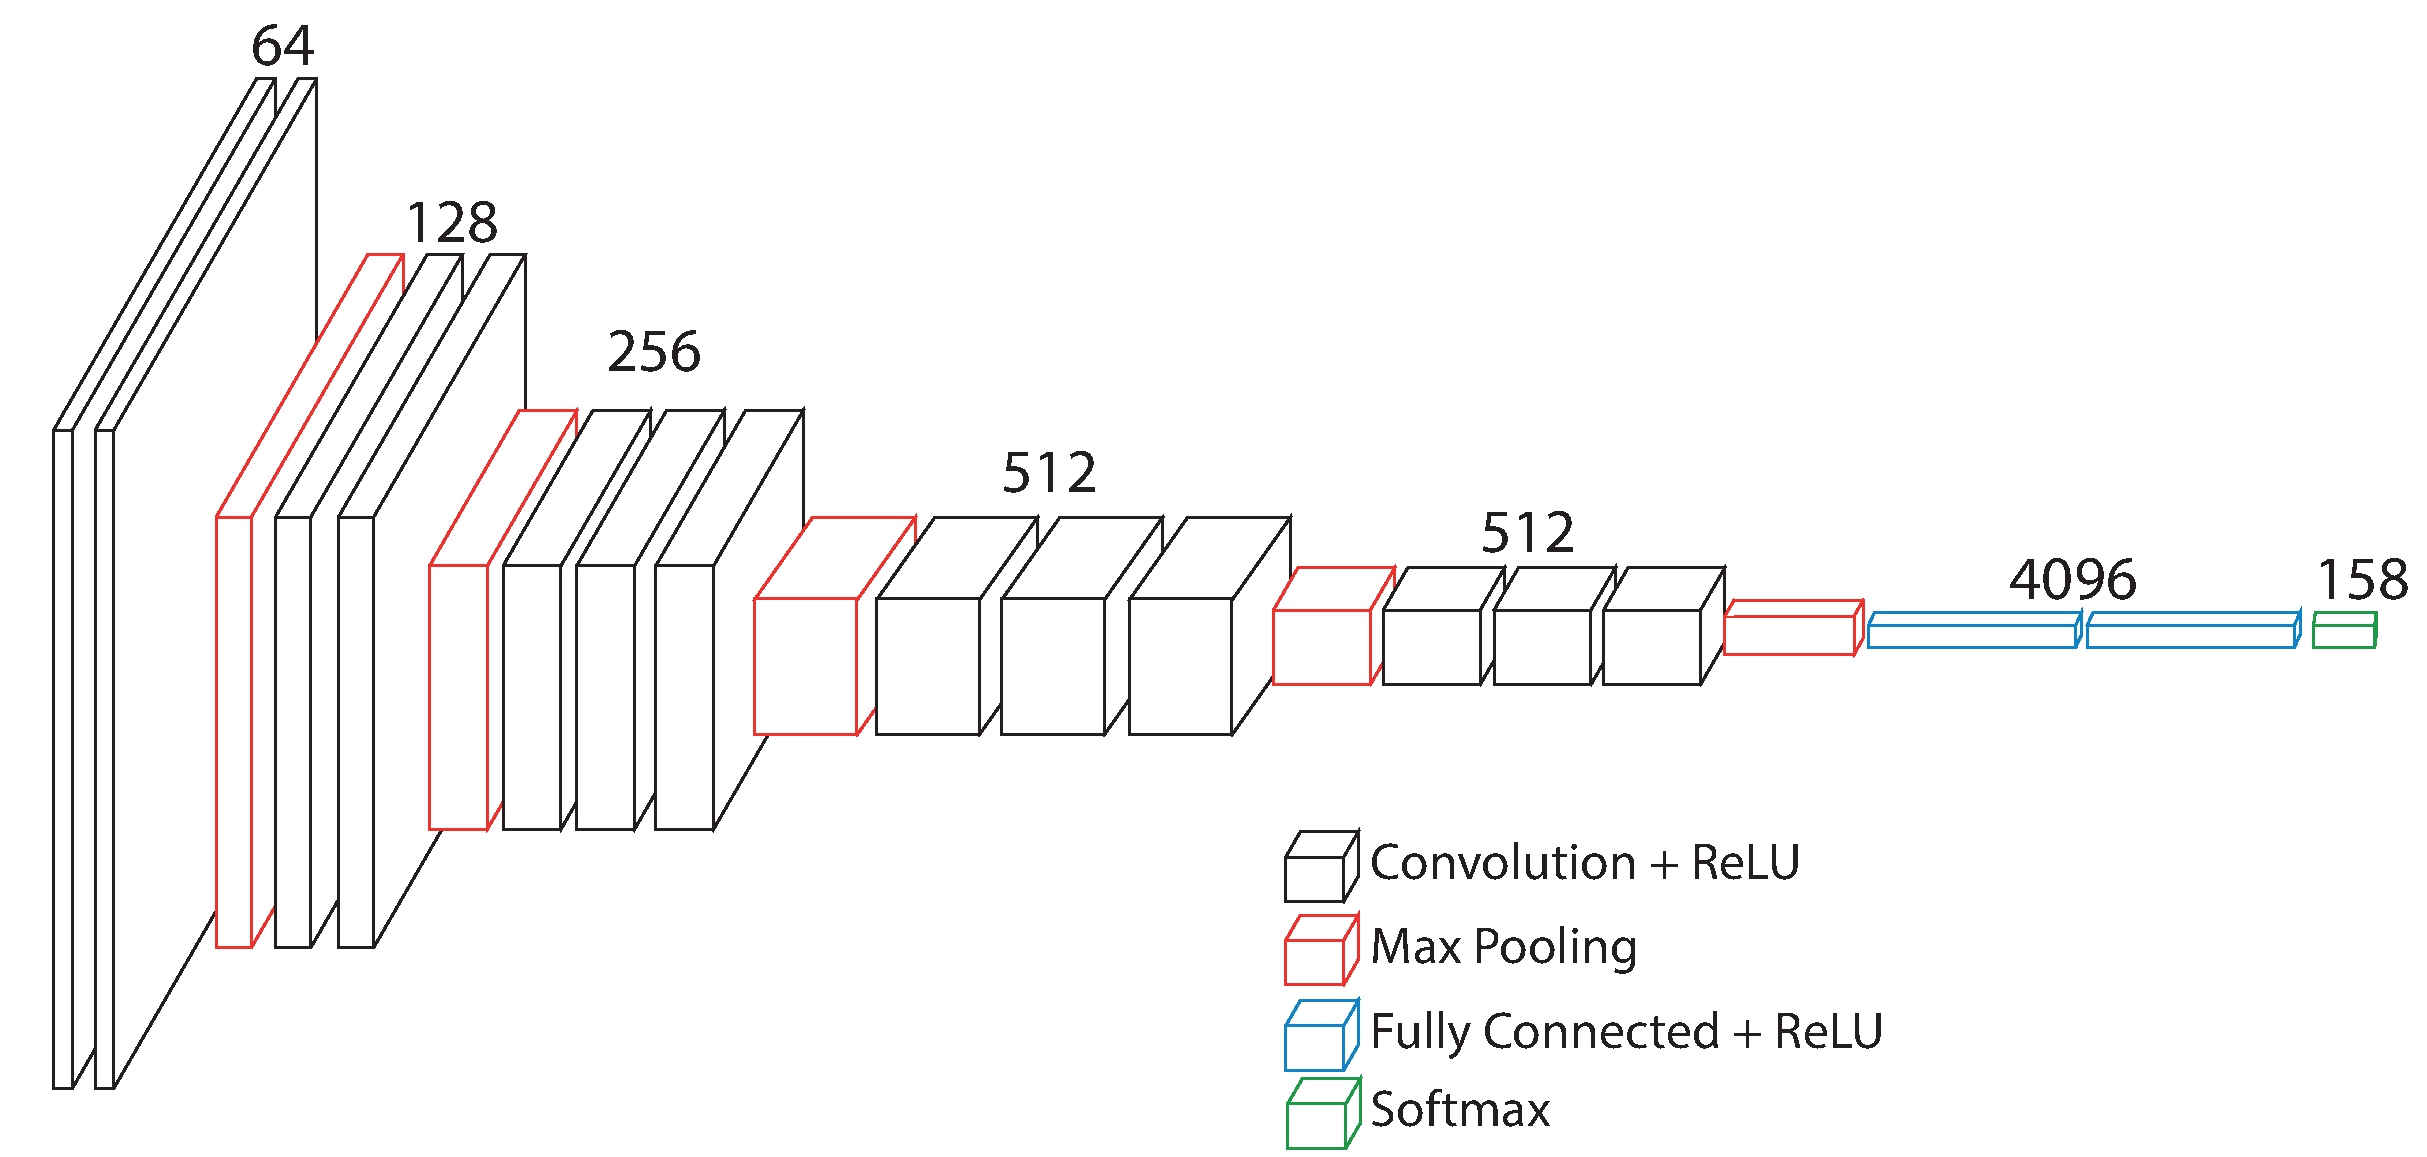
\includegraphics[width=\textwidth]{vgg16_overview}
	\caption{Overview of the VGG16 \gls{cnn} used for face recognition. Only the depth of the layers is known and noted. The input is excluded from the figure.}
	\label{fig:vgg16}
\end{figure}

\begin{table}[H]
	\centering
	\caption{Detailed description of VGG16 design. The input is $64\times64\times3$ images.}
	\label{tab:vgg16}
	\begin{tabular}{lrrrr}
		\textbf{Layer Type}     & \textbf{Feature Map Size} & \textbf{Kernel/Pool Size} & \textbf{Activation} & \textbf{Other} \\ \hline
		\textbf{Block 1}        &                           &                           &                     &                \\
		\rowcolor{lightGrey}  
		Conv2D                  & $64$                      & $3\times3$                & ReLU                &                \\
		Conv2D                  & $64$                      & $3\times3$                & ReLU                &                \\
		\rowcolor{lightGrey} 
		MaxPooling2D            &                           & $2\times2$                &                     &                \\
		\textbf{Block 2}        &                           &                           &                     &                \\
		\rowcolor{lightGrey}  
		Conv2D                  & $128$                     & $3\times3$                & ReLU                &                \\
		Conv2D                  & $128$                     & $3\times3$                & ReLU                &                \\
		\rowcolor{lightGrey}  
		MaxPooling2D            & $2\times2$                & $5\times5$                & ReLU                &                \\
		\textbf{Block 3}        &                           &                           &                     &                \\
		\rowcolor{lightGrey}  
		Conv2D                  & $256$                     & $3\times3$                & ReLU                &                \\
		Conv2D                  & $256$                     & $3\times3$                & ReLU                &                \\
		\rowcolor[HTML]{EFEFEF} 
		Conv2D                  & $256$                     & $3\times3$                & ReLU                &                \\
		MaxPooling2D            & $2\times2$                &                           &                     &                \\
		\textbf{Block 4}        &                           &                           &                     &                \\
		\rowcolor{lightGrey}  
		Conv2D                  & $512$                     & $3\times3$                & ReLU                &                \\
		Conv2D                  & $512$                     & $3\times3$                & ReLU                &                \\
		\rowcolor{lightGrey}  
		Conv2D                  & $512$                     & $3\times3$                & ReLU                &                \\
		MaxPooling2D            & $2\times2$                &                           &                     &                \\
		\textbf{Block 5}        &                           &                           &                     &                \\
		\rowcolor{lightGrey}  
		Conv2D                  & $512$                     & $3\times3$                & ReLU                &                \\
		Conv2D                  & $512$                     & $3\times3$                & ReLU                &                \\
		\rowcolor{lightGrey}  
		Conv2D                  & $512$                     & $3\times3$                & ReLU                &                \\
		MaxPooling2D            & $2\times2$                & $3\times3$                & ReLU                &                \\
		\textbf{Classification} &                           &                           &                     &                \\
		\rowcolor{lightGrey}  
		Flatten                 &                           &                           &                     &                \\
		Dense                   & $4096$                    &                           & ReLu                &                \\
		\rowcolor{lightGrey}  
		Dropout                 &                           &                           &                     & $0.5$          \\
		Dense                   & $4096$                    &                           & ReLu                &                \\
		\rowcolor{lightGrey} 
		Dropout                 &                           &                           &                     & $0.5$          \\
		Dense                   & Amount of Classes         &                           & Softmax             &               
	\end{tabular}
\end{table}

\begin{figure}[H]
	\centering
	\begin{subfigure}{0.48\textwidth}
		\centering
		\includegraphics[width=\textwidth]{vgg16_acc}
		\caption{Face recognition \gls{cnn} accuracy progression through epochs}
		\label{fig:vgg16_acc}
	\end{subfigure}
	\begin{subfigure}{0.48\textwidth}
		\centering
		\includegraphics[width=\textwidth]{vgg16_loss}
		\caption{Face recognition \gls{cnn} loss progression through epochs}
		\label{fig:vgg16_loss}
	\end{subfigure}
	\caption{Accuracy and loss progression for the face recognition VGG16 \gls{cnn}.}
	\label{fig:vgg_graphs}
\end{figure}

\section{Network Fusion}
To be able to combine iris and face verification, a combination of the results of the two networks is made.  This is done by having two individual streams that are merged at their last \gls{fc} layer by concatenating the layers along their longest dimension. The merged layer can then be fed into other \gls{fc} layers and further to a classification layer. This is done using a softmax layer after the \gls{fc} layer \citep{Eitel2015}. This should in theory increase the accuracy in ID verification in a potential instance where verification is required. The architecture used is shown in \autoref{fig:net_fusion}. The two \gls{fc} has 5020 neurons. This is to have the same dimensions as the concatenated layer. To see if the new merged structure performs better than the iris and face \gls{cnn}s separately, the same hyper parameters are used as earlier in this chapter.

\begin{figure}[h]
	\centering
	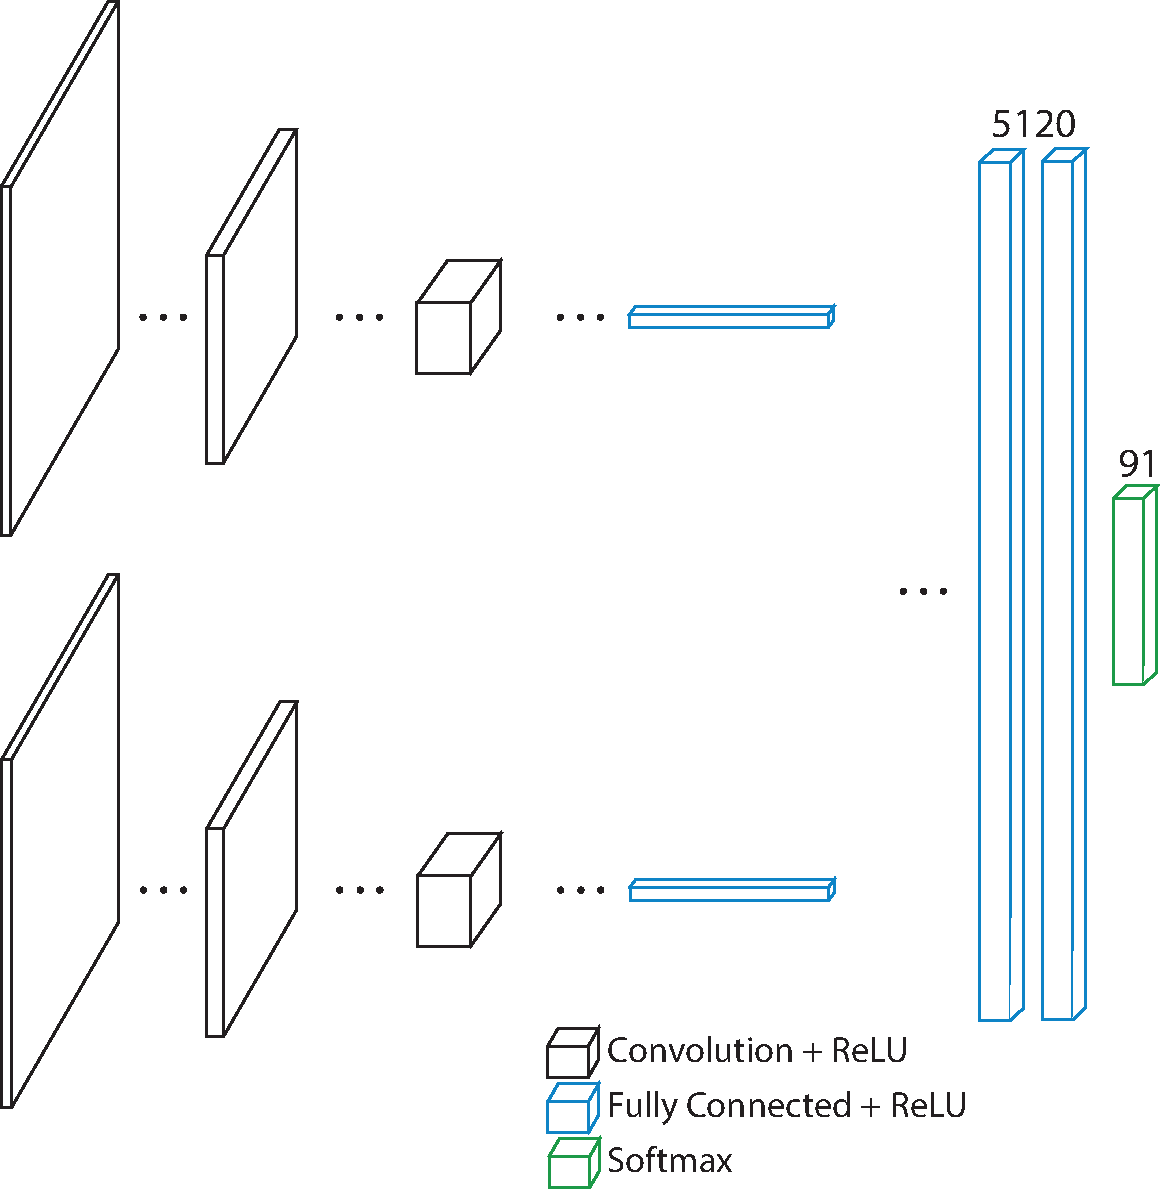
\includegraphics[width=0.8\textwidth]{merged_net_overview}
	\caption{Overview of how the two networks are fused}
	\label{fig:net_fusion}
\end{figure}

The parameters set for classification in the fused network are shown in \autoref{tab:merged_net}

\begin{table}[h]
	\centering
	\caption{Parameters set for the classification in the fused network}
	\label{tab:merged_net}
	\begin{tabular}{lrrrr}
		\textbf{Layer Type} & \textbf{Feature Map Size} & \textbf{Kernel/Pool Size} & \textbf{Activation} & \textbf{Other} \\ \hline
		\multicolumn{5}{l}{Iris Recognition and Face Recognition Networks Outputs}                                        \\
		\rowcolor{lightGrey}
		Concatenate         &                           &                           &                     &                \\
		Dense               & $5120$                    &                           & ReLU                &                \\
		\rowcolor{lightGrey} 
		Dropout             &                           &                           &                     & $0.5$          \\
		Dense               & $5120$                    &                           & ReLU                &                \\
		\rowcolor{lightGrey} 
		Dropout             &                           &                           &                     & $0.5$          \\
		Dense               & Amount of Classes         &                           &  Softmax            &               
	\end{tabular}
\end{table}

%To be able to reuse as much as possible, the two databases used with the networks separately are also used in the fusion of the networks instead of using a multimodal database as presented in \autoref{cha:Research}. This means that a combination of the two databases is necessary as the data have not been collected by the same groups or from the same people. The databases does not have the same amount of classes, therefore the larger database is reduced also reducing the entire amount of usable data.

\subsection{Multimodal Database}
The fusion net should be trained with a multimodal biometric database. Ideally the database used in this project should consist of face and iris images obtained from the same subjects captured with the same camera complying with the requirements set in \autoref{ch:req}. 

However, even though literature suggests that chimeric databases are less adequate than genuine multimodal biometric databases, the multimodal database used during the work with information fusion is synthetically created. As \autoref{sec:multi_modal_data} mentions there are only a limited amount of multimodal biometric databases available containing both iris and face data, and, to the extend of the knowledge gained from the research presented in \autoref{sec:info_fuse}, there is only one of the databases, which is obtained using mobile devices namely the MobBio database. For this database the Asus Transformer Pad TF 300T is used, which has a camera of 8MP, and is thus comparable to the iPhone 5s used for the caption of the Warsaw-BioBase used for the iris identification methods presented in \autoref{BasicM} and \autoref{sec:cnn_iris_rec} \citep{Sequeira2014}. However, despite several attempts of contacting the authors of the database it was not possible to establish communication or gain access to the database. Therefore the available way to obtain a multimodal database with mobile device images is to create it synthetically. Furthermore as the goal is to compare the performance of the fused \gls{cnn}s with the individual \gls{cnn}s on the face and iris data respectively, it is desirable to test on the same data. Therefore a databased was created by combining the \gls{lfw} and the Warsaw-BioBase databases. 

The database was created by combining iris classes arbitrarily with an face class for as many classes as there were classes available from both the iris and the face dataset. Before combining the datasets the classes with ten or less samples were discarded. The new samples were made by giving the iris image and the face image the same label. The new samples were then data augmented as described in \autoref{sec:cnn_iris_rec}

\subsection{Results}
The chimera database consists of 20640 samples across 91 classes. 70\% was used for training, 15\% for validation and 15\% for testing. The network was trained for 140 epochs and achieved a test accuracy of 81.17\%

\begin{figure}[H]
	\centering
	\begin{subfigure}{0.48\textwidth}
		\centering
		\includegraphics[width=\textwidth]{merged_acc_81_17_acc}
		\caption{Face recognition \gls{cnn} accuracy progression through epochs}
		\label{fig:merged_acc}
	\end{subfigure}
	\begin{subfigure}{0.48\textwidth}
		\centering
		\includegraphics[width=\textwidth]{merged_acc_81_17_loss}
		\caption{Face recognition \gls{cnn} loss progression through epochs}
		\label{fig:merged_loss}
	\end{subfigure}
	\caption{Accuracy and loss progression for the merged \gls{cnn}. Achieved 81.17\% accuracy on the test set}
	\label{fig:merged_graphs}
\end{figure}

\noindent As the merged \gls{cnn} using the chimera data performed worse by almost 20\% something was wrong. To investigate how the separate iris and face \gls{cnn}s would perform on the chimera data a second test was made. This was done by simply discarding either the iris or the face respectively from the generated sample. This produced the following result with the same 70, 15, 15 split.  The iris \gls{cnn} achieved 68.94\% accuracy on the test set, \autoref{fig:iris_cnn_68_graphs}. The VGG face \gls{cnn} achieved 77.78\% accuracy on the test set, \autoref{fig:vgg_77_graphs}. When all networks used the same data the merged network seems to outperform both the VGG face \gls{cnn} and the iris \gls{cnn} although they both achieved above 99\% accuracy when trained on the data before the it was fused to the chimera data.

\begin{figure}[H]
	\centering
	\begin{subfigure}{0.48\textwidth}
		\centering
		\includegraphics[width=\textwidth]{iris_cnn_bad_68_94_acc}
		\caption{Iris \gls{cnn} accuracy progression through epochs}
		\label{fig:iris_cnn_68_acc}
	\end{subfigure}
	\begin{subfigure}{0.48\textwidth}
		\centering
		\includegraphics[width=\textwidth]{iris_cnn_bad_68_94_loss}
		\caption{Iris \gls{cnn} loss progression through epochs}
		\label{fig:iris_cnn_68_loss}
	\end{subfigure}
	\caption{Accuracy and loss progression for the iris \gls{cnn} trained on chimera data. Achieved 68.94\% accuracy on the test set.}
	\label{fig:iris_cnn_68_graphs}
\end{figure}


\begin{figure}[H]
	\centering
	\begin{subfigure}{0.48\textwidth}
		\centering
		\includegraphics[width=\textwidth]{vgg16_bad_77_88_acc}
		\caption{Face recognition \gls{cnn} accuracy progression through epochs}
		\label{fig:vgg_77_acc}
	\end{subfigure}
	\begin{subfigure}{0.48\textwidth}
		\centering
		\includegraphics[width=\textwidth]{vgg16_bad_77_88_loss}
		\caption{Face recognition \gls{cnn} loss progression through epochs}
		\label{fig:vgg_77_loss}
	\end{subfigure}
	\caption{Accuracy and loss progression for the VGG face \gls{cnn} trained on chimera data. Achieved 77.78\% accuracy on the test set }
	\label{fig:vgg_77_graphs}
\end{figure}


%\graphicspath{{figures/test/}}
\chapter{Tests}

%\chapter{Conclusion}\label{ch:conclusion}\glsresetall
Throughout the project, the work has been aimed at finding a solution to the problem statement; \\
\textbf{How well can identity verification be performed on \gls{vl} smart phone images of iris and face, and to which extend can the performance be improved by information fusion?}

To be able to perform identity verification on smart phone images of iris and face, several recognition solutions was made.

Iris recognition was done in multiple ways. Firstly, different regular machine learning solutions was made. The best performance was using a polynomial kernel for \gls{svm}, with an accuracy of $98\%$ which did not meet the requirement set for the accuracy.
Therefore, a deep learning solution was introduced. By using a \gls{cnn} with a total of 14 layers, it was possible to achieve an accuracy of $99.7\%$, which satisfied the requirement of at least $99\%$ accuracy. 
Both the machine learning and deep learning solution used the Warsaw BioBase database, a database with close-up photos of irises captured with an Apple iPhone 5s.

Face recognition was made using a pre-made image classification model, VGG16. This model is pre-trained on the ImageNet database with 2000 different classes, and the weights from this are used in the implementation of the model. The \gls{cnn} used the \gls{lfw} database and achieved an accuracy of $99.35\%$, which also satisfied the requirement of accuracy limit.

A fusion of the two successful \gls{cnn}s was then made. For this network, the databases used with the two separate networks was combined into one database with a label for an iris and a face tying them together. This network achieved an accuracy of $81.17\%$, which is not better than any of the stand-alone networks.

% For use if report is split up in parts
\bookmarksetup{startatroot}% Goto root of Table of Contents
\addtocontents{toc}{\bigskip}% Add space before next item in Table of Contents

% Appearance of the bibliography
\iflanguage{english}{%
\bibliographystyle{setup/plainnat_en}%
}{%
\bibliographystyle{setup/plainnat_dk}%
}
\label{LastPage}


\bibliography{bib/VGIS8.bib}
\label{bib:mybiblio}




%\setlength{\chapnumb}{2cm} % Ændrer længden på stregen under kapiteloverskriften så den passer til bilag
\appendix % Start of appendix
\addtocontents{toc}{\protect\setcounter{tocdepth}{0}} 


\end{document}
